\documentclass{article}
\usepackage[utf8]{inputenc}
\usepackage{booktabs}
\usepackage{graphicx}
\usepackage{float}
\title{Rocket Stage Optimization Results}
\author{Generated by Stage\_Opt}
\date{\today}

\begin{document}
\maketitle

\section{Introduction}
This report presents the results of optimizing a two-stage rocket using various optimization methods. The objective was to minimize the payload mass fraction while satisfying the total delta-V requirement.

\section{Optimization Results}
\begin{table}[H]
\centering
\begin{tabular}{lccr}
\toprule
Method & Payload Fraction & Error & Time (s) \\
\midrule
SLSQP & 0.0000 & 0.0000e+00 & 0.00 \\
BASIN-HOPPING & 0.0000 & 3.3451e-09 & 0.28 \\
GA & 0.0000 & 0.0000e+00 & 0.00 \\
ADAPTIVE-GA & 0.0000 & 0.0000e+00 & 0.00 \\
DE & 0.0000 & 0.0000e+00 & 0.00 \\
PSO & 0.0068 & 1.8190e-12 & 0.26 \\
\bottomrule
\end{tabular}
\caption{Summary of optimization results}
\label{tab:results}
\end{table}

\section{Figures}
\begin{figure}[H]
\centering
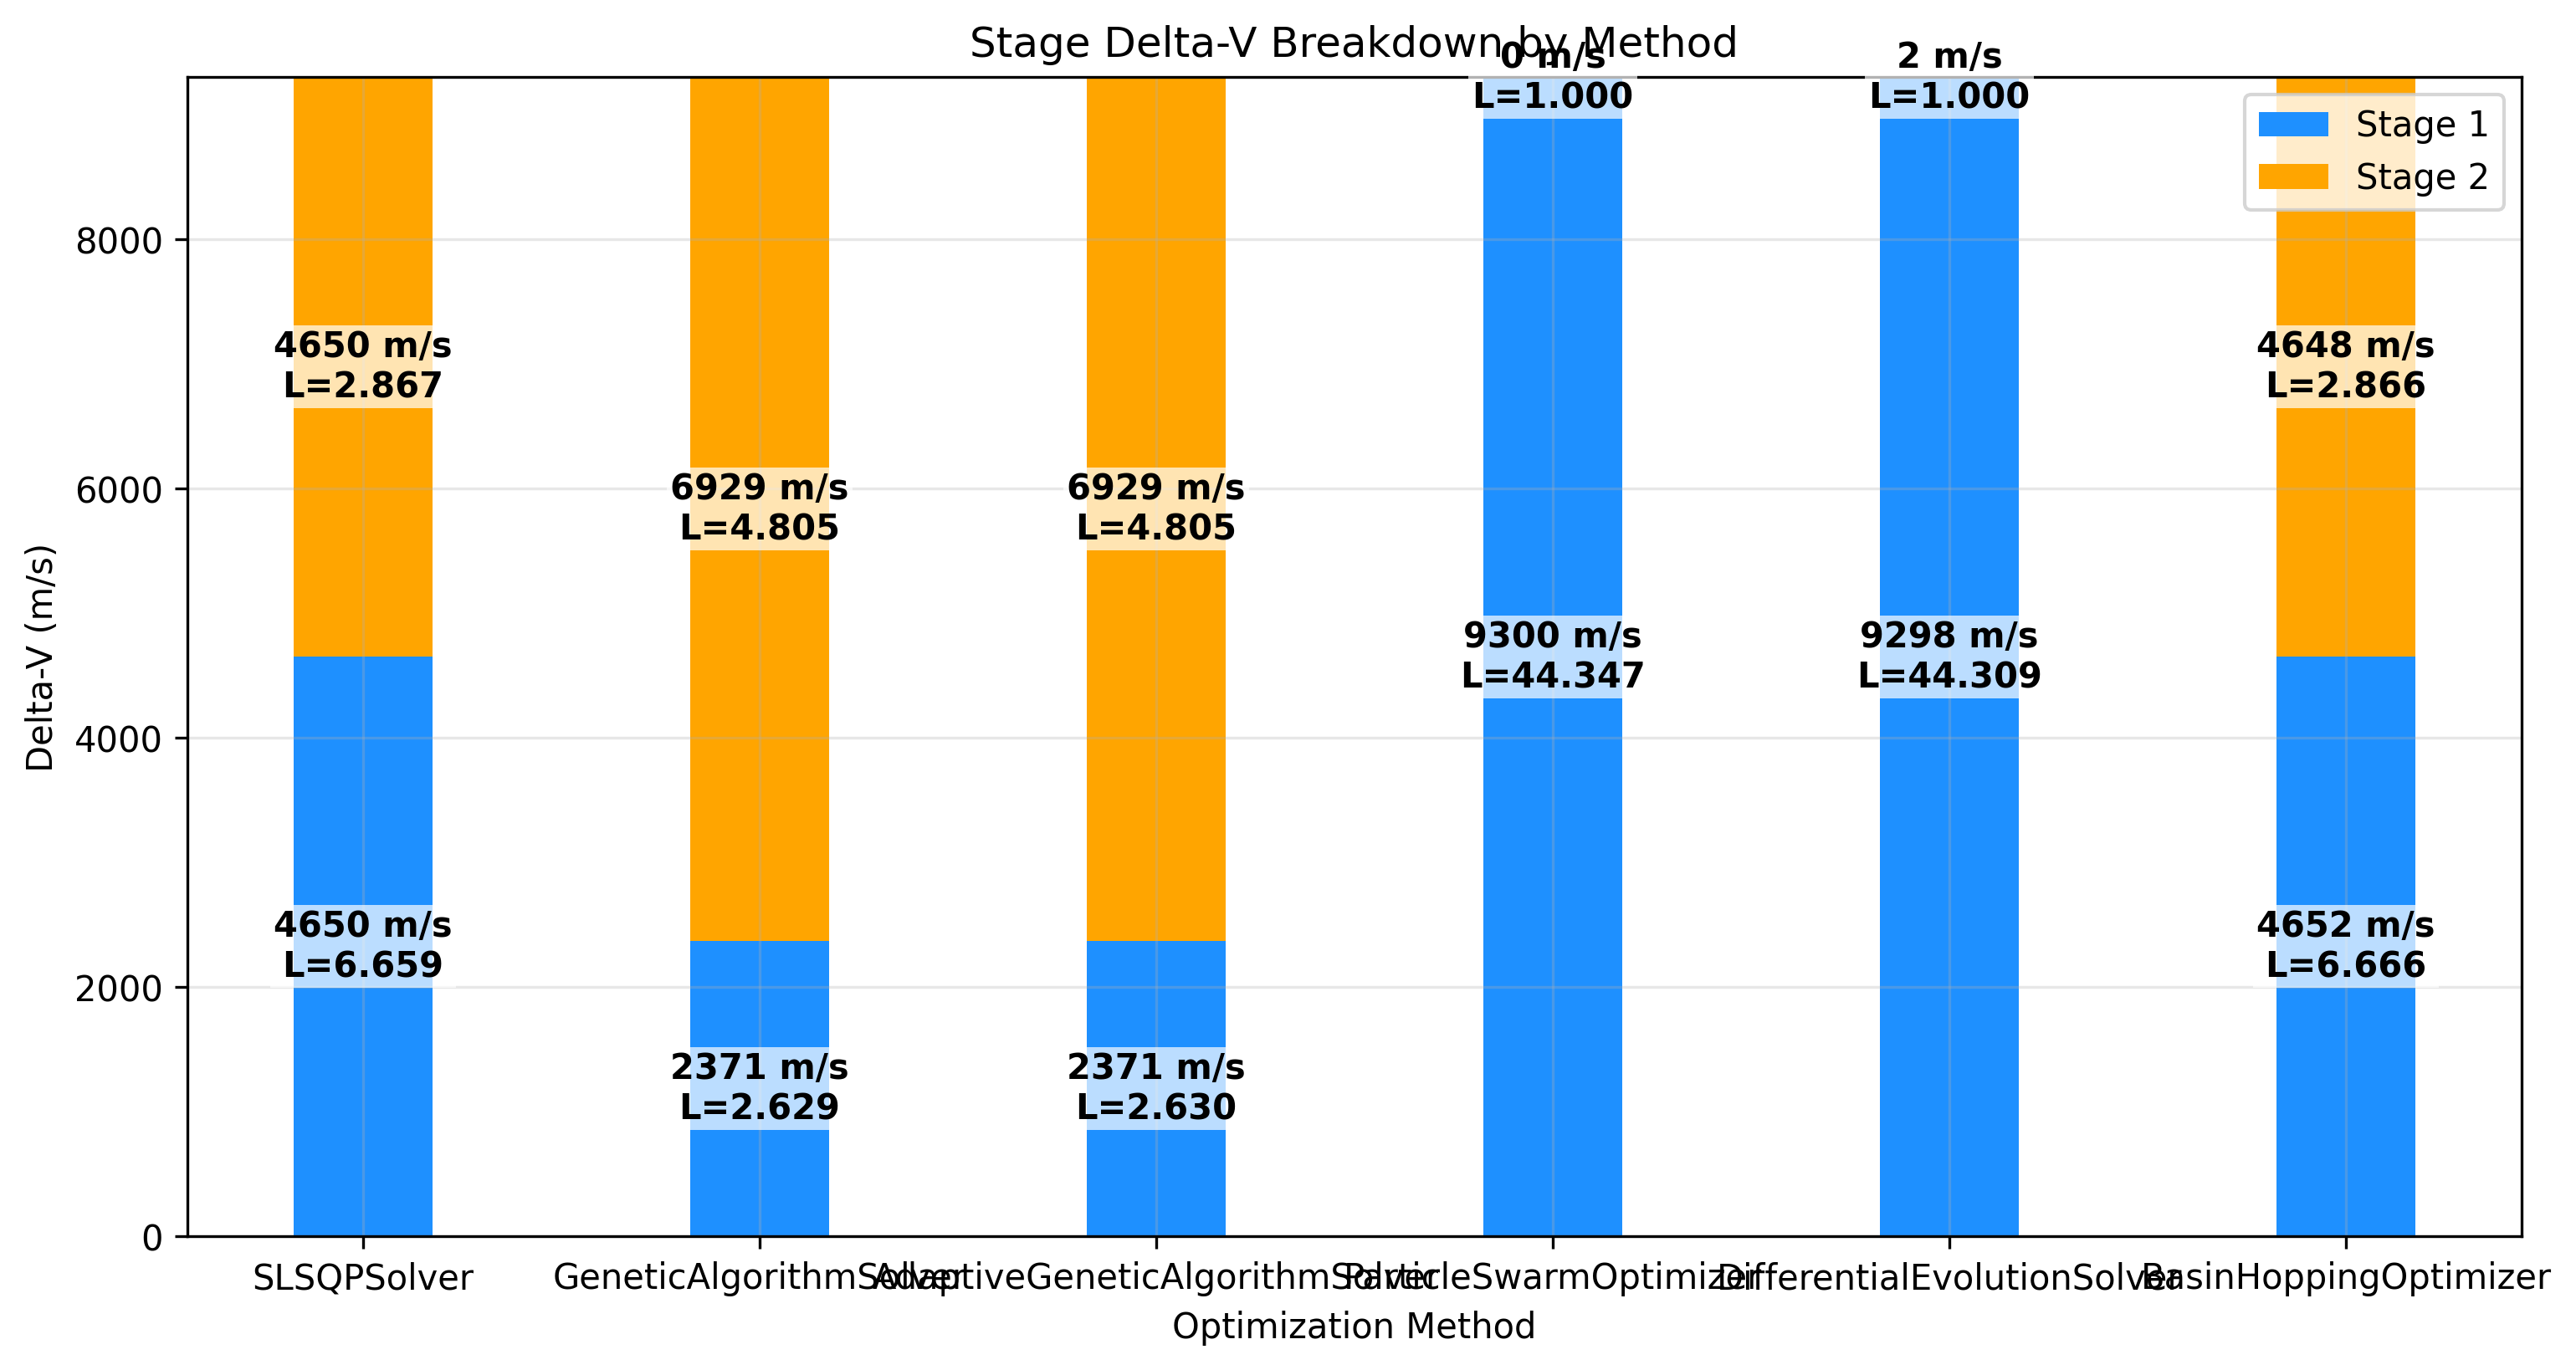
\includegraphics[width=\textwidth]{dv_breakdown.png}
\caption{Delta-V distribution across stages for each optimization method}
\label{fig:dv-breakdown}
\end{figure}

\begin{figure}[H]
\centering
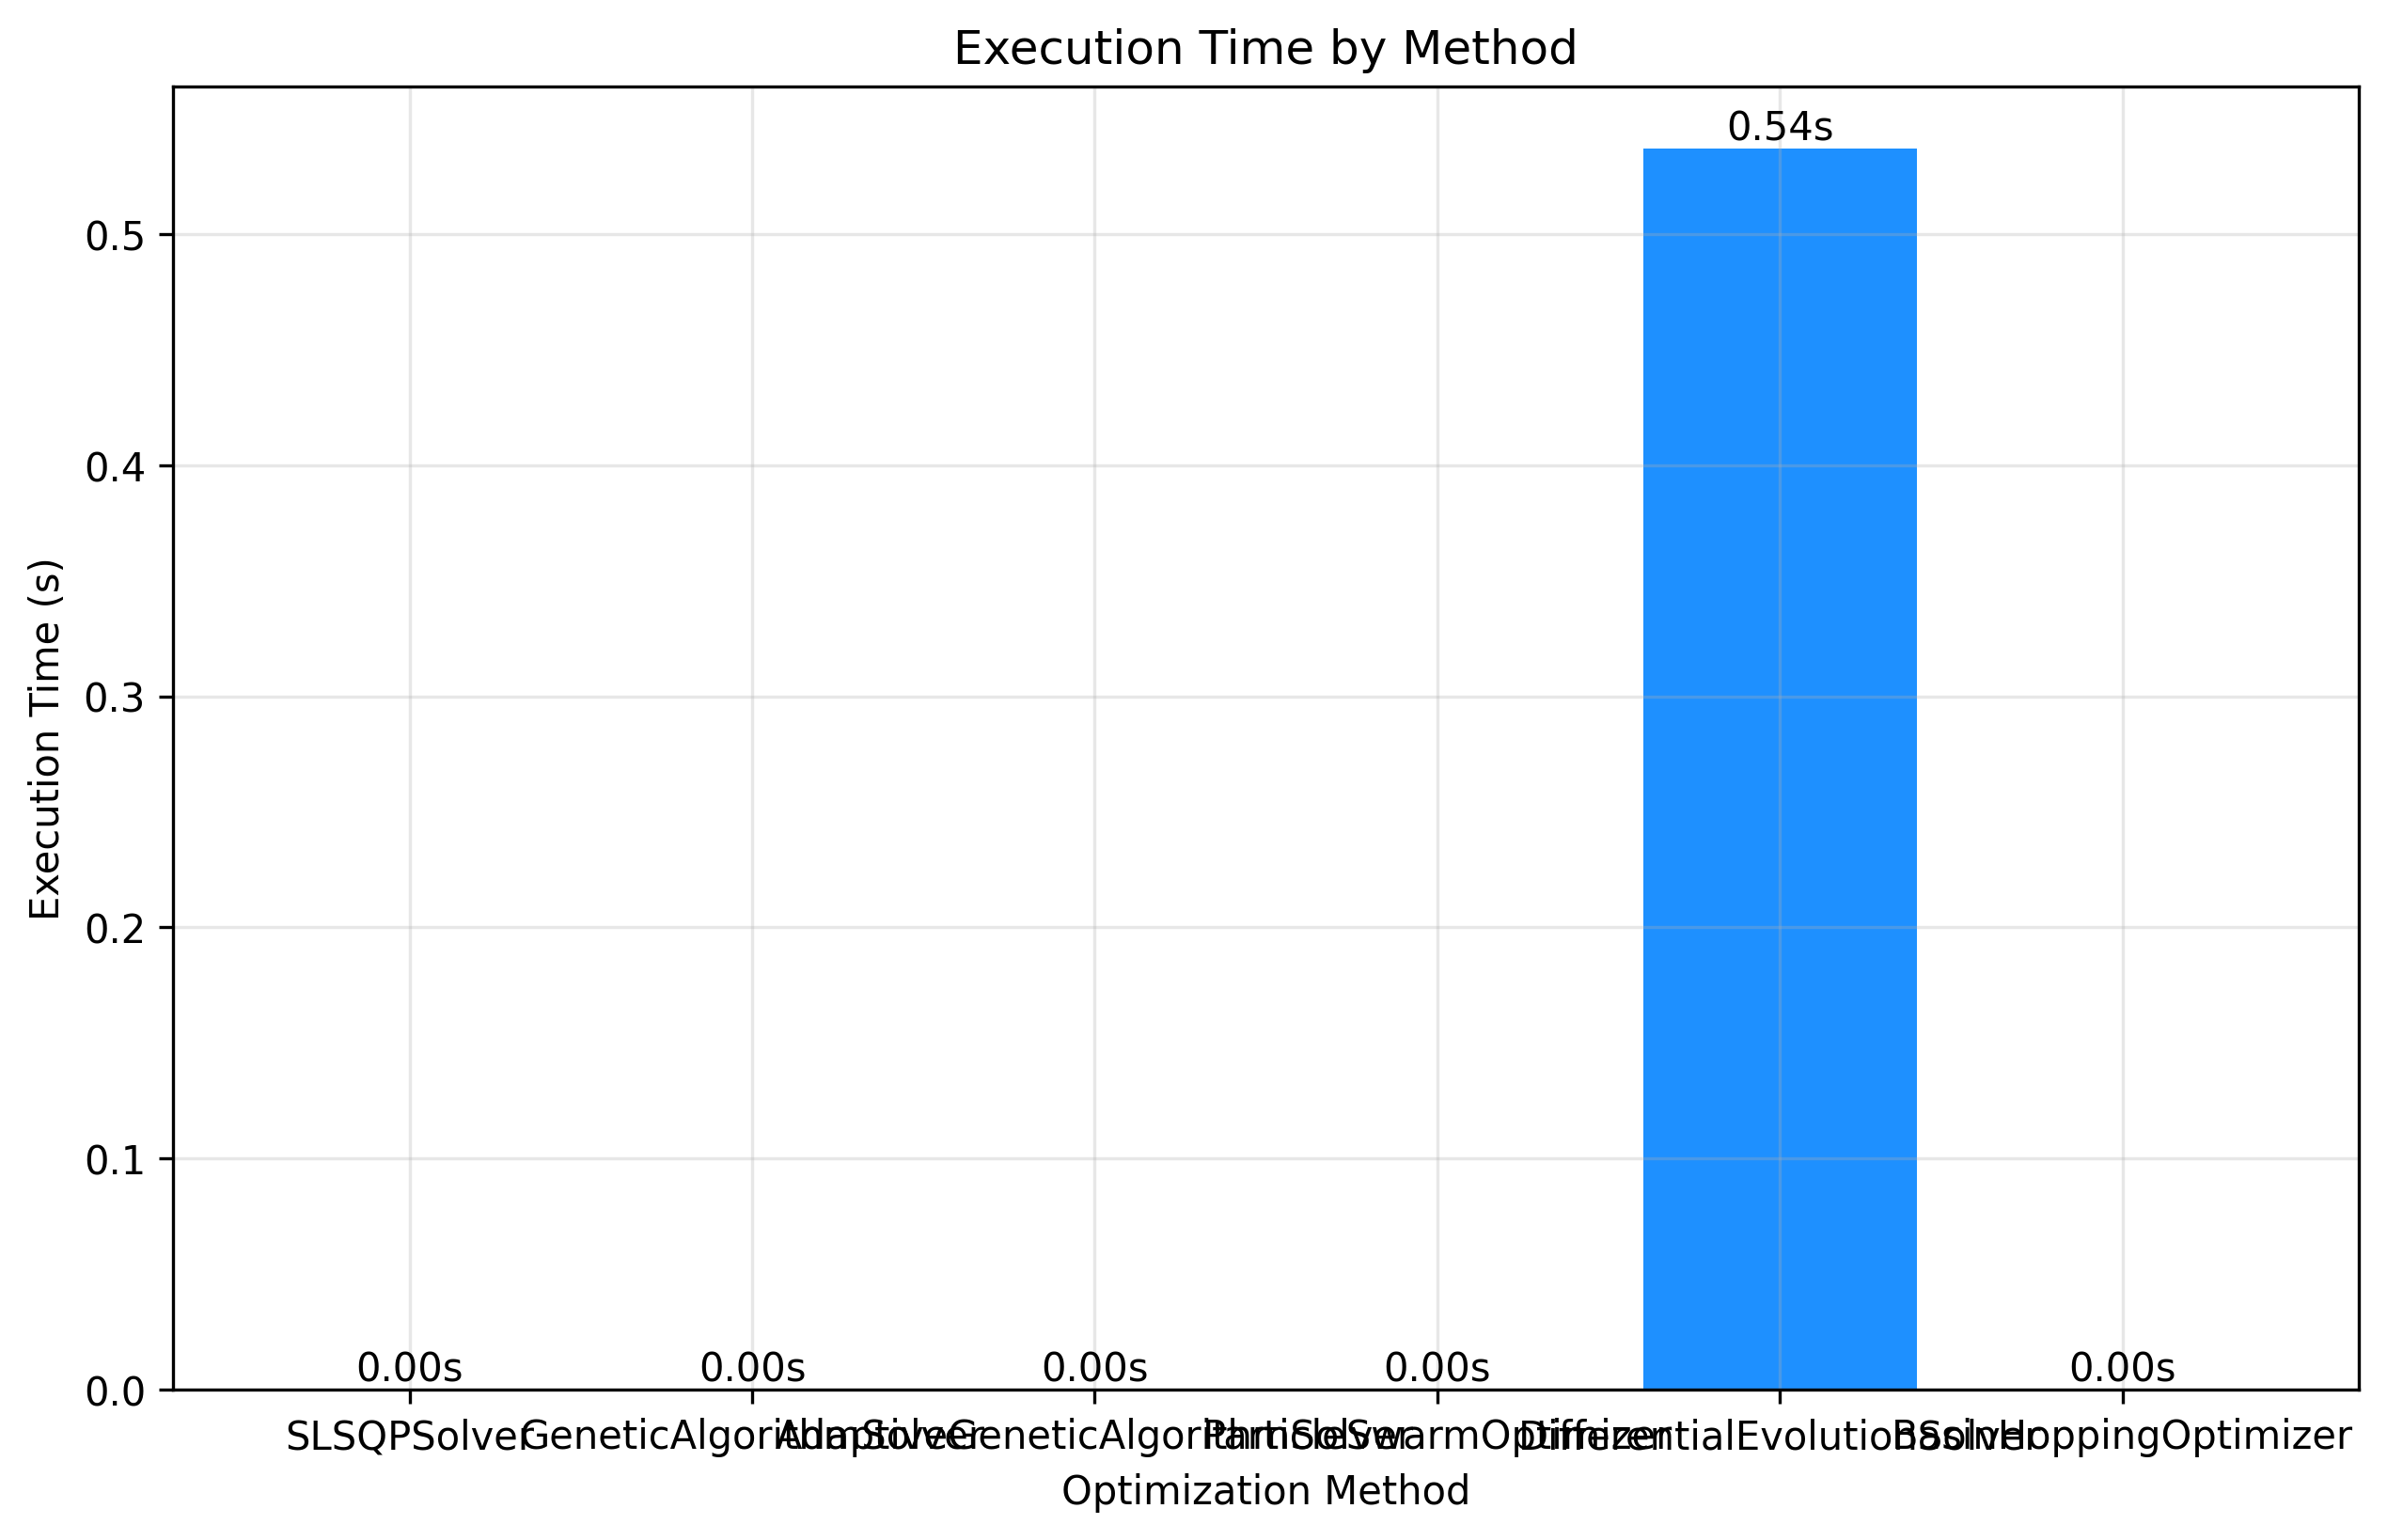
\includegraphics[width=\textwidth]{execution_time.png}
\caption{Execution time comparison across optimization methods}
\label{fig:execution-time}
\end{figure}

\begin{figure}[H]
\centering
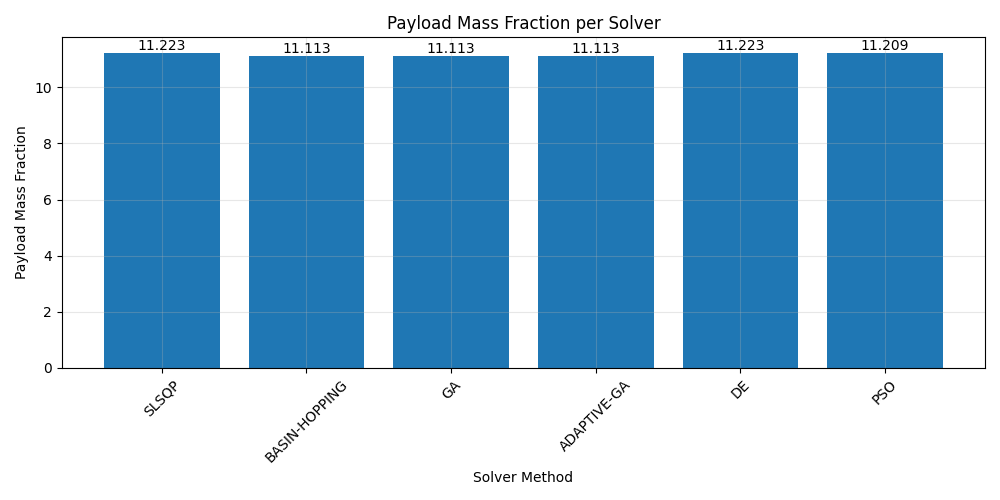
\includegraphics[width=\textwidth]{payload_fraction.png}
\caption{Payload fraction comparison across optimization methods}
\label{fig:payload-fraction}
\end{figure}

\section{Conclusion}
The optimization results show that the PSO method achieved the best performance with a payload fraction of 0.0068. This suggests that PSO is most suitable for this particular rocket stage optimization problem.

\end{document}
